\section{Improving Recognition Accuracy}
%\frame{\tableofcontents[currentsection, currentsubsection]}
\frame{\tableofcontents[currentsection]}

\frame{ \frametitle{Improved Face Window} 
\centering
\begin{tabular}{@{}cc@{}}
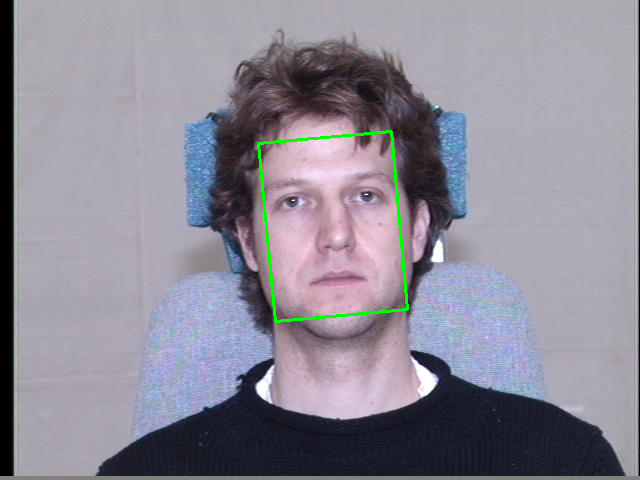
\includegraphics[trim=1.9in .7in 1.9in .5in, clip, height=1.1in]{../figures_pami/example.png} &
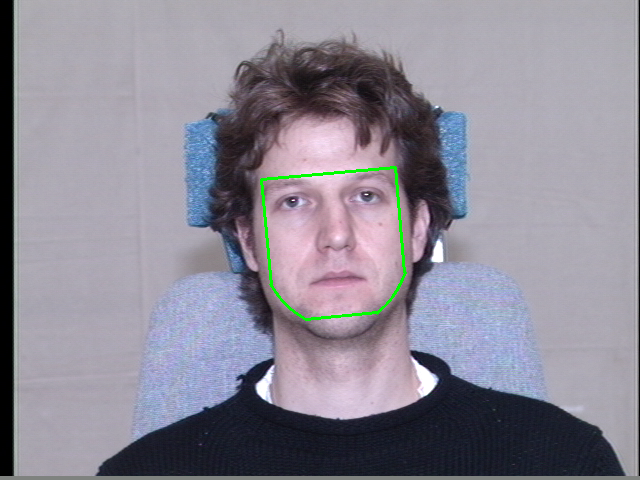
\includegraphics[trim=1.9in .7in 1.9in .5in, clip, height=1.1in]{../figures_pami/example_new.png} \\
Default window. & Proposed window.
\end{tabular}

{Recognition rates on the Multi-PIE database
 %and [Yang2010-CVPR]
}
\centerline{
\begin{tabular}{|c|c|c|c|c| }
\hline
Recognition rate & Session 2 & Session 3 & Session 4  \\
\hline
%{Alg. 1, $S=1$} & 90.7\% & 89.6\% & 87.5\% \\
%\hline
{Rectangular Window} & 93.9\% & 93.8\% & 92.3\% \\
\hline
{Improved window} & 95.0\% & {\bf 96.3}\% & {\bf 97.3}\% \\
\hline
%\cite{Yang2010-CVPR} & {\bf 95.2}\% & 93.4\% & 95.1\% \\
%\hline
\end{tabular}
} }

\frame{ \frametitle{Centering the test image before recognition} 
\begin{itemize}
\item After iterative alignment, test and training images can be transformed
together as a set without breaking the model.
\item In first prototype, test image was kept at initial (face detector) position.
\item In second prototyte, average of alignments is used to better position test
image in window.
\item In both prototypes, training images stay aligned relative to test image.
\item Fewer background pixels in the frame.
\end{itemize}
}

\frame{ \frametitle{Difficulty with MRF Model} 
\begin{itemize} 
\item Success! MRF improves occlusion handling for the aligned case.
\item When MRF model and iterative alignment are combined,
alignment stability problems arise.  
\item The core problem: unable to differentiate error caused by occlusion and
error caused by initial misalignment. 
\item Need occlusion model that don't destabilize alignment.
\end{itemize}
}

\frame{ \frametitle{Overlapping Block Model} 
\centering
{
	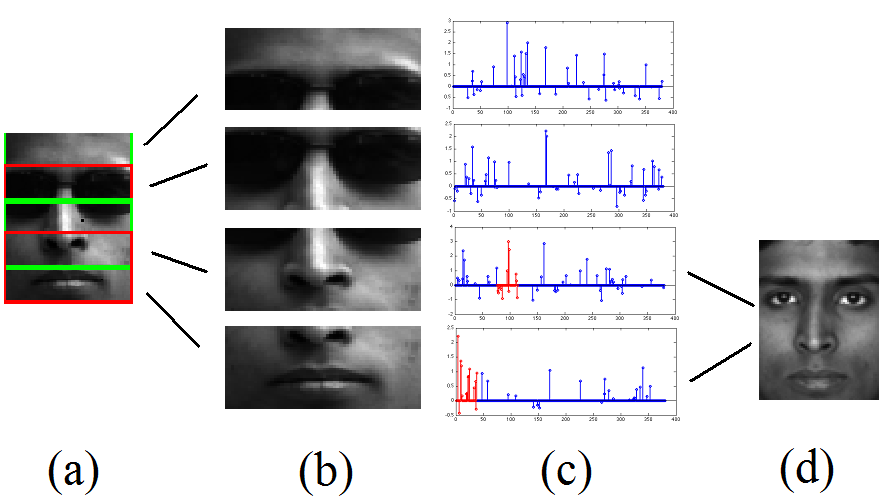
\includegraphics[width=3in]{../figures_pami/occ_block.png}
}
\begin{itemize} \item Want to better handle sunglasses
\item Perform recognition {\em independently} on a set of \newline reduced size overlapping blocks that are:
\begin{itemize}
\item small enough to sometimes miss occlusions
\item large enough to converge independently
\end{itemize}
\item...and vote to complete the classification.
\end{itemize}
}

\newcommand{\tempwidth}{0.1667\textwidth}
\frame{ \frametitle{Robustness to Sunglasses} 
\centering
\begin{tabular}{@{}c@{}c@{}c@{}c@{}c@{}c@{}}
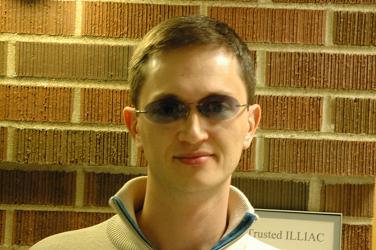
\includegraphics[width=\tempwidth,clip=true]{../figures_pami/uiuc_example/sunglasses/DSC_1565.JPG} &
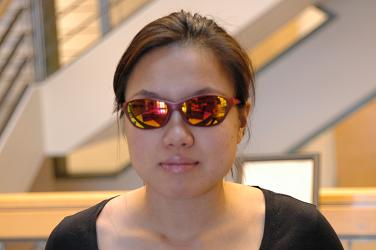
\includegraphics[width=\tempwidth,clip=true]{../figures_pami/uiuc_example/sunglasses/DSC_3656.JPG} &
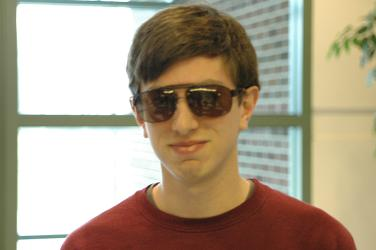
\includegraphics[width=\tempwidth,clip=true]{../figures_pami/uiuc_example/sunglasses/DSC_3827.JPG} &
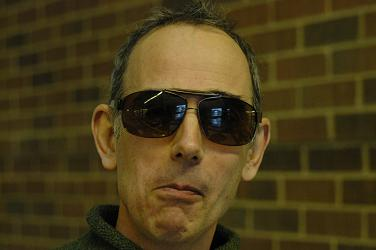
\includegraphics[width=\tempwidth,clip=true]{../figures_pami/uiuc_example/sunglasses/DSC_4090.JPG} &
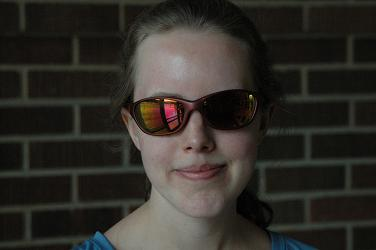
\includegraphics[width=\tempwidth,clip=true]{../figures_pami/uiuc_example/sunglasses/DSC_4106.JPG} &
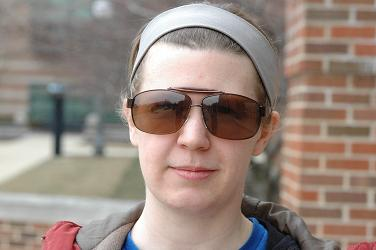
\includegraphics[width=\tempwidth,clip=true]{../figures_pami/uiuc_example/sunglasses/DSC_4126.JPG} \\
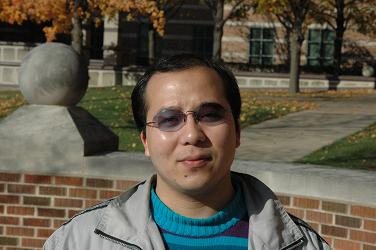
\includegraphics[width=\tempwidth,clip=true]{../figures_pami/uiuc_example/sunglasses_failed/DSC_1611.JPG} &
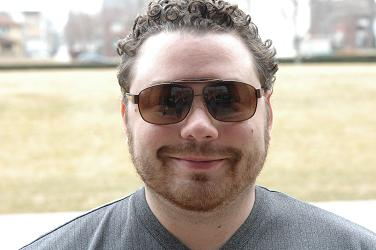
\includegraphics[width=\tempwidth,clip=true]{../figures_pami/uiuc_example/sunglasses_failed/DSC_3528.JPG} &
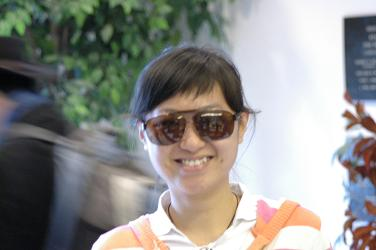
\includegraphics[width=\tempwidth,clip=true]{../figures_pami/uiuc_example/sunglasses_failed/DSC_3744.JPG} &
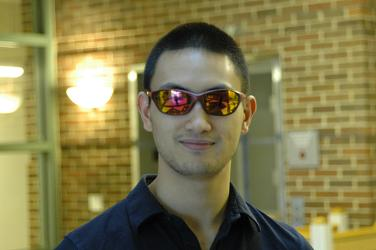
\includegraphics[width=\tempwidth,clip=true]{../figures_pami/uiuc_example/sunglasses_failed/DSC_3995.JPG} &
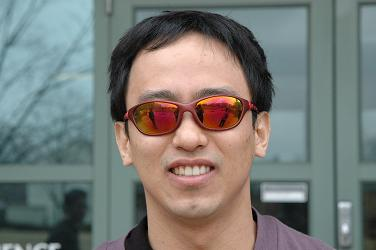
\includegraphics[width=\tempwidth,clip=true]{../figures_pami/uiuc_example/sunglasses_failed/DSC_4030.JPG} &
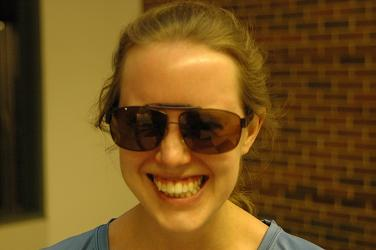
\includegraphics[width=\tempwidth,clip=true]{../figures_pami/uiuc_example/sunglasses_failed/DSC_4095.JPG} \\
\end{tabular}
Top row: examples where the overlapping blocks method succeeded. 
Bottom row: examples where the overlapping blocks method failed.
}

\frame{\frametitle{Large Scale Experiments}
\begin{itemize}
\item Recognition rates on the Multi-PIE session 1 
\item Different pairings of alignment and recognition stages
\end{itemize}
\centering
\begin{tabular}{|c|c|c|c|}
\hline
\backslashbox{Rec.}{Align.} & Face Detector & Manual & Iterative \\
\hline
NS	& 30.8\%	& 77.6\%	& 84.5\%	\\
\hline
NN	& 26.4\%	& 67.3\%	& 73.5\%	\\
\hline
LDA	& 5.1\%		& 49.4\%	& 91.0\%	\\
\hline
LBP	& 39.9\%	& 93.3\%	& {\bf 95.2\%}	\\
\hline
SRC	Prototype 1& -- & -- & 91.4\%	\\
\hline
SRC	Prototype 2& -- & -- & 93.9\%	 \\
\hline
\end{tabular}
\begin{itemize}
\item Our iterative alignment algorithm improves all algorithms tested!
\item Second prototype pipeline shows improved performance!
\end{itemize}
}

\frame{ \frametitle{Impostor Rejection} 
\centerline{
\begin{tabular}{@{}cc@{}}
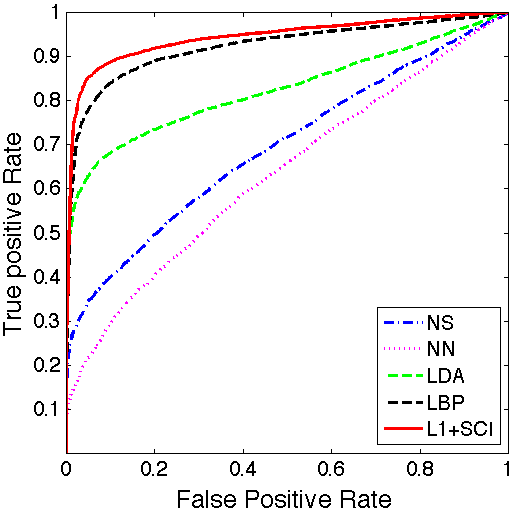
\includegraphics[height=1.5in]{../figures_pami/pami_roc_revision2} &
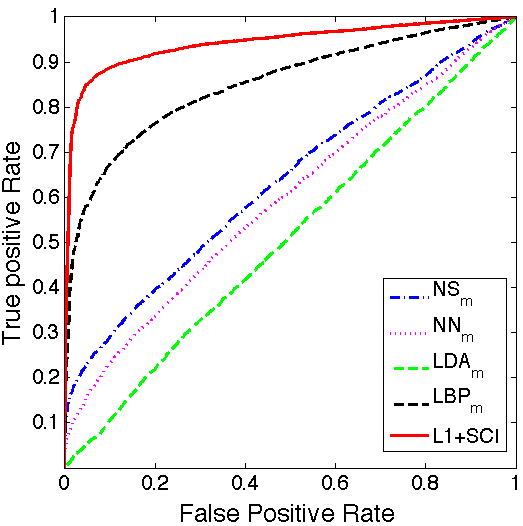
\includegraphics[height=1.5in]{../figures_pami/pami_roc2} \\
(a) & (b) \\
\end{tabular}
}
(a) Iterative alignment for all agorithms \newline
(b) The classical algorithms with manual alignment (indicated by a subscript ``m'').

\begin{itemize}
\item Again, iterative alignment helps in all cases
\item SRC based pipeline still better at rejecting impostors!
\end{itemize}
}

%\frame{ \frametitle{Improved performance on private dataset}
%Recognition rates on a more realistic private database.
%\begin{tabular}{|c|c|c|c|c|}
%\hline
%Test Category & C1 & C2 & C3 & C4  \\
%\hline
%\hline
%Recognition Rate & 98.4\% & 95.8\% & 95.1\% & 40.9\% \\
%\hline
%\end{tabular}
%}

